\documentclass[11pt,letterpaper]{article}
\usepackage[margin=0.62in,top=0.69in,bottom=0.66in,headheight=15pt,headsep=13pt,footskip=24pt]{geometry}
\usepackage{tikz,amsmath,amssymb,fancyhdr,array}
\usetikzlibrary{arrows.meta}
\usepackage[T1]{fontenc}\usepackage{lmodern}
\renewcommand{\familydefault}{\sfdefault}
\pagestyle{fancy}\fancyhf{}\fancyhead[L]{\small Week 70 / Shields in a portal room / Grades 4--5}
\fancyfoot[L]{\scriptsize Bellingham Math Circle / Week 70 / GGT70-S-v2}\fancyfoot[R]{\scriptsize\thepage}
\renewcommand{\headrulewidth}{0.4pt}\renewcommand{\footrulewidth}{0pt}
\setlength{\parindent}{0pt}\setlength{\parskip}{8pt}
\newcommand{\problem}[2]{\textbf{Problem #1:} #2\par}

\newcommand{\room}[3][]{% [extra TikZ code] scale, arrow choice 0 none 1 NE 2 NW 3 SE 4 SW
\begin{tikzpicture}[scale=#2]
\draw[step=1,gray!28,thin] (0,0) grid (4,4);
\draw[thick] (0,0) rectangle (4,4);
\foreach\p in {(0,0),(4,0),(0,4),(4,4)}{\fill\p circle(1.7pt);}
\node[below left,font=\small]at(0,0){S};\node[below right,font=\small]at(4,0){S};
\node[above left,font=\small]at(0,4){S};\node[above right,font=\small]at(4,4){S};
\fill[white](2,2)circle(4pt);\draw[thick](2,2)circle(3pt);\node[above right,font=\small]at(2,2){T};
\node[below,font=\scriptsize]at(2,0){Y};\node[above,font=\scriptsize]at(2,4){Y};
\node[left,font=\scriptsize]at(0,2){X};\node[right,font=\scriptsize]at(4,2){X};
\ifnum#3=1\draw[-{Stealth[length=5pt]},very thick](0,0)--(.65,.65);\fi
\ifnum#3=2\draw[-{Stealth[length=5pt]},very thick](4,0)--(3.35,.65);\fi
\ifnum#3=3\draw[-{Stealth[length=5pt]},very thick](0,4)--(.65,3.35);\fi
\ifnum#3=4\draw[-{Stealth[length=5pt]},very thick](4,4)--(3.35,3.35);\fi
#1
\end{tikzpicture}}
\newcommand{\mapwindow}[2][.70]{% [scale] extra TikZ code
\begin{tikzpicture}[scale=#1]
\draw[step=1,gray!23,thin](-4,-4)grid(12,12);
\foreach\x in{-4,0,4,8,12}{\draw[gray!75,line width=.7pt](\x,-4)--(\x,12);}
\foreach\y in{-4,0,4,8,12}{\draw[gray!75,line width=.7pt](-4,\y)--(12,\y);}
\foreach\x in{-2,2,6,10}{\foreach\y in{-2,2,6,10}{\draw[fill=white,thick](\x,\y)circle(2.6pt);\node[above right,font=\scriptsize]at(\x,\y){T};}}
\fill(0,0)circle(3pt);\node[below right,fill=white,inner sep=1pt,font=\small]at(0,0){S};
\draw[line width=1.2pt](0,0)rectangle(4,4);
\foreach\x in{-4,0,4,8,12}{\node[below,font=\scriptsize]at(\x,-4){\x};}
\foreach\y in{-4,0,4,8,12}{\node[left,font=\scriptsize]at(-4,\y){\y};}
#2
\end{tikzpicture}}
\newcommand{\lines}[1]{\foreach\n in{1,...,#1}{\noindent\rule{\linewidth}{.2pt}\par\vspace{.22in}}}
\begin{document}

A shot travels straight. At an X edge it reappears at the same height on the other X edge. Y edges work the same way, at the same left-to-right position. It keeps its direction. All four corners are the same S. Stop at the first T reached.

A shield is one exact point, away from S and T, marked with a small pencil cross. A shield stops a shot only if the shot passes exactly through that point. On an unfolded map, each large square is another copy of the same room, and every T is the same target. A shield repeats at the same place in every copy.

\begin{center}
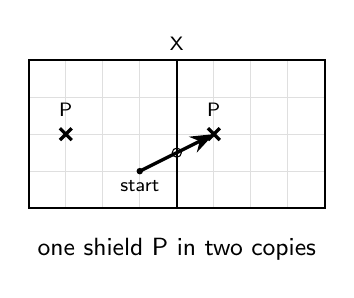
\begin{tikzpicture}[scale=.47]
\draw[step=1,gray!25](0,0)grid(8,4);\draw[thick](0,0)rectangle(4,4);\draw[thick](4,0)rectangle(8,4);
\fill(3,1)circle(2.5pt);\draw[-{Stealth},very thick](3,1)--(5,2);\draw(4,1.5)circle(3.5pt);
\foreach\x in{1,5}{\draw[very thick](\x-.16,1.84)--(\x+.16,2.16);\draw[very thick](\x-.16,2.16)--(\x+.16,1.84);\node[above,font=\scriptsize]at(\x,2.2){P};}
\node[below,font=\scriptsize]at(3,1){start};\node[above,font=\scriptsize]at(4,4){X};
\node[below,font=\small]at(4,-.55){one shield P in two copies};
\end{tikzpicture}\hspace{.35in}
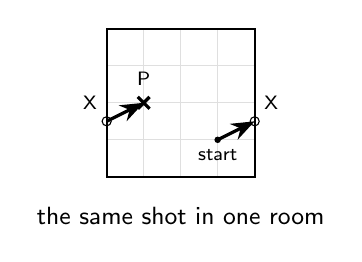
\begin{tikzpicture}[scale=.47]
\draw[step=1,gray!25](0,0)grid(4,4);\draw[thick](0,0)rectangle(4,4);
\fill(3,1)circle(2.5pt);\draw[-{Stealth},very thick](3,1)--(4,1.5);\draw[-{Stealth},very thick](0,1.5)--(1,2);
\draw[very thick](.84,1.84)--(1.16,2.16);\draw[very thick](.84,2.16)--(1.16,1.84);\node[above,font=\scriptsize]at(1,2.2){P};
\draw(0,1.5)circle(3.5pt);\draw(4,1.5)circle(3.5pt);
\node[below,font=\scriptsize]at(3,1){start};\node[left,font=\scriptsize]at(0,2){X};\node[right,font=\scriptsize]at(4,2){X};
\node[below,font=\small]at(2,-.55){the same shot in one room};
\end{tikzpicture}
\end{center}

\problem{1}{Finish the four diagonal shots. Choose one shield arrangement for the room that stops all six shots. Use as few shields as you can. Your partner checks the shot lines and shields.}

\begin{center}
\room[{\foreach\a/\b/\c/\d in{0/0/.65/.65,4/0/3.35/.65,0/4/.65/3.35,4/4/3.35/3.35}{\draw[-{Stealth[length=6pt]},very thick](\a,\b)--(\c,\d);}
\draw[thick,-{Stealth[length=5pt]}](0,0)--(4/3,4);\draw[thick,-{Stealth[length=5pt]},shorten >=4pt](4/3,0)--(2,2);
\draw[thick,-{Stealth[length=5pt]}](0,0)--(4,4/3);\draw[thick,-{Stealth[length=5pt]},shorten >=4pt](0,4/3)--(2,2);
\foreach\p in{(4/3,4),(4/3,0),(4,4/3),(0,4/3)}{\draw\p circle(3.5pt);}}]{1.9}{0}
\end{center}
\vfill
Our fewest shields: \rule{.9in}{.3pt}

\newpage

\problem{2}{Aim straight shots from S at the T copies A $(2,6)$, B $(6,2)$, C $(6,6)$ and D $(10,6)$. Your partner marks the first T each shot reaches. In the small room, draw one shot that crosses an X or Y edge before reaching T.}

\begin{center}\mapwindow[1.0]{\foreach\x/\y/\l in{2/6/A,6/2/B,6/6/C,10/6/D}{\node[below right,font=\small\bfseries]at(\x,\y){\l};}}\end{center}
\begin{center}\room{1.0}{0}\end{center}

\newpage

\problem{3}{Find four shield points in the bold room that stop every shot on the map. Your partner chooses targets and uses straight shots on the map to test your shields. Move your shields until no shot gets through.}

\begin{center}\mapwindow[1.05]{}\end{center}

\newpage

\problem{4}{Find four shield points that stop every straight shot from S to T, even one that goes far beyond the map. Explain why your points work. Could three shields ever stop every shot?}

\vspace{.15in}
\begin{center}\room{1.65}{0}\end{center}
\vspace{.20in}\lines{5}

\end{document}
